%\documentclass[]{article}
\documentclass[a4paper]{article}

\usepackage[paperheight=11in,paperwidth=8.5in,top=.7in,bottom=.7in,right=.5in,left=.5in,heightrounded]{geometry}
 
\usepackage{amsmath}
\numberwithin{equation}{subsection}

%\usepackage{boondox-cal}
\usepackage{parskip} % For no paragraph indentation
\usepackage{xcolor}

\DeclareMathOperator{\sinc}{sinc}


\usepackage{fancyhdr}
\pagestyle{fancy}
%\rhead{Engr. Muhammad Abu Bakar Siddique}
%\rhead{\thepage}
\lhead{
\includegraphics[height=1cm]{../figures/Tajdar2.png}}
\rhead{
\includegraphics[height=1cm]{../figures/Labbaik1.png}}
\chead{\thepage}
%\lhead{RCET, UET Lahore}
\cfoot{}

\usepackage{graphicx}

\usepackage{chngcntr}
\counterwithin{figure}{section}

%opening
\title{Digital Transmission through Bandlimited AWGN Channels}
\author{Engr. Muhammad Abu Bakar Siddique}

\begin{document}
	
	\maketitle
%	
%	\begin{abstract}
%		
%	\end{abstract}
	
	
	%\counterwithin{figure}{section}
	\setcounter{section}{8}
	%\subsection*{Introduction}
	
	\begin{figure}[h] 
		
\includegraphics[width=.7\textwidth]{../figures/darood}	
		\centering
	\end{figure}

	\vspace{-1.5em}
	
	\setcounter{figure}{0}
	\subsection{Pulse Amplitude Modulation in AWGN}
	
	Binary modulations are good to transmit digital data. However, their one drawback is we can send only one binary digit in a signal waveform. To transmit multiple bits per signal, we make use of M-ary modulation. In M-ary modulation we use $M$ pulse instead of only two, hence increasing the number of bits per signal. Now let us explore the Pulse Amplitude Modulation (PAM) which is the first example of M-ary modulation.
	\
	\begin{itemize}
		\item No. of pulse levels in binary modulation is TWO
		\item No. of pulse levels in PAM is $M$, 
		\item Binary modulation becomes special case of PAM with $M=2$
		\item No. of bits per pulse is $k=\log_2 M$
		\item Each pulse has a waveform $s_m(t)$, where $m=\{1,2,\dots,M\}$
		\item All pulses are level shifted version of basic pulse $p(t)$
		
		
	\end{itemize}
	
	\begin{figure}[!hbt]
		\centering
		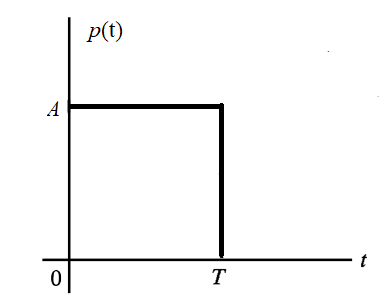
\includegraphics[width=2in]{../figures/fig8_5}
		\caption{The basic pulse $p(t)$}
		\label{fig:fig85}
	\end{figure}
	
	
	\begin{equation}\label{eq:pt}
	p(t) = \left\{\begin{array}{cc}
	A, & 0\leq t < T  \\
	0, & \text{otherwise}
	\end{array}   \right..
	\end{equation}
	
	\begin{figure}
		\centering
		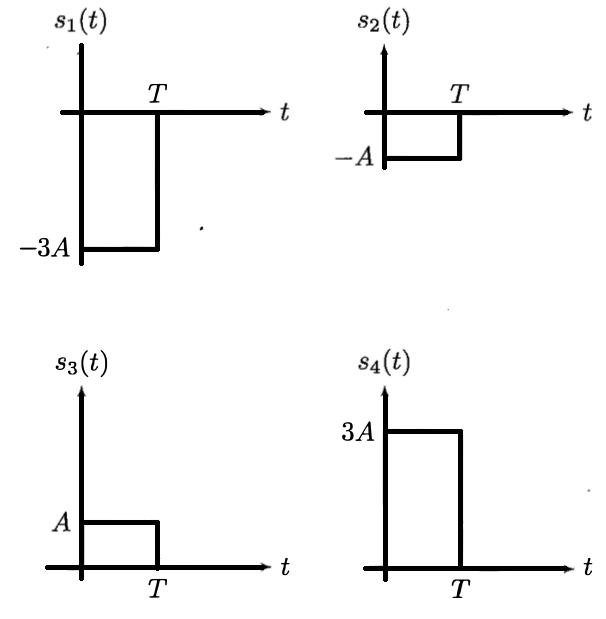
\includegraphics[width=3in]{../figures/fig8_42}
		\caption{The 4-PAM pulses with amplitudes $-3A,-A,A$ and $3A$. Here M=4 is used.}
		\label{fig:fig8_42}
	\end{figure}
	
	
	So the other pulses are level shifted version of $p(t)$
	
	\begin{equation}\label{key}
	s_m(t)=A_m p(t), \quad m=1,2,\cdots,M
	\end{equation}
	
	The basic pulse has magnitude $A$. 
	
	The magnitudes of $M$ pulses are
	
	\begin{equation}\label{key}
	[-(M-1), \cdots, -3,-1, 1, 3, \cdots, (M-1)]A
	\end{equation}
	
	
	In total there are $M$ levels from $-(M-1)A$ to $(M-1)A$ in increments of 2A.
	
	The most negative pulse $s_1(t)$ has amplitude multiplier $A_1 = -(M-1)$ 
	
	The highest positive pulse $s_M(t)$ has amplitude multiplier $A_M = (M-1)$ 
	
	So an arbitrary pulse $s_m(t)$ has amplitude multiplier $A_m$
	
	\begin{equation}\label{eq:am}
	A_m = (2m-M-1), \quad m=1,\cdots,M
	\end{equation}
	
	To find orthonoraml basis we apply Gram-Schmidt algorithm. It is easier if we start with the pulse having amplitude $A$, that is the pulse $p(t)$ defined in Equation (\ref{eq:pt}).
	
	%and is the $\frac{2+M}{2}$th pulse
	
	So the first orthonormal basis is
	
	\begin{equation}\label{key}
	\psi(t)=\frac{p(t)}{\mathcal{E}_p}
	\end{equation}
	Now we calculate energy of $p(t)$
	
	\begin{align}\label{key}
	\mathcal{E}_p&= \int_0^\infty (p(t))^2 dt \nonumber \\
	&= \int_0^T A^2 dt \nonumber \\
	&= A^2 |t|_0^T \nonumber \\
	&= A^2 T
	\end{align}
	So the basis function is 
	
	\begin{equation}\label{key}
	\psi(t)=\frac{p(t)}{A\sqrt{T}}
	\end{equation}
	
	\begin{figure}
		\centering
		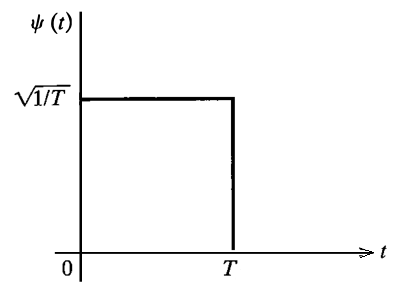
\includegraphics[width=2in]{../figures/fig8_7a}
		\caption{The basis functions obtaind from normalizing $p(t)$ by its energy.}
		\label{fig:fig8_7a}
	\end{figure}
	
	
	The good news is that it is the only basis function and all other signals lie parallel to this basis. It can be proved in few lines
	
	\subsubsection*{There is just one orthonormal basis}
	
	Let us take an arbitrary waveform $s_m(t)$ and othonormalize it to $\psi(t)$. First calculate the correlation $s_{m}$ between $s_m(t)$ and $\psi(t)$ as 
	
	\begin{equation}
	\begin{aligned}\label{eq:sm}
	s_{m}&=\int_{-\infty}^\infty s_m(t)\psi(t) dt \\
	&= \int_{-\infty}^\infty (A_m p(t) ) (\frac{p(t)}{A\sqrt{T}})\\
	&= \frac{A_m}{A\sqrt{T}} \int_{-\infty}^\infty (p(t))^2 dt \\
	&= \frac{A_m}{A\sqrt{T}} \int_0^T (A)^2 dt \\
	%&= \frac{A^2 A_m}{A\sqrt{T}} |t|_0^T \\
	&= \frac{A^2 A_m}{A\sqrt{T}} T \\
	&= A A_m \sqrt{T} \\
	%&= (2m-1-M)A\sqrt{T} 
	\end{aligned}
	\end{equation}
	
	The orthogonal part $d_m(t)$ of $s_m(t)$ is calculated by subtracting from $s_m(t)$ its projection along $\psi(t)$.
	
	\begin{equation}\label{key}
	\begin{aligned}
	d(t)&= s_m(t)-s_{m}\psi(t)\\
	&= s_m(t)-A A_m \sqrt{T} \frac{p(t)}{A\sqrt{T}}\\
	&= s_m(t)-A_m p(t) \\
	&= s_m(t)-s_m(t) \\
	&= 0
	\end{aligned}
	\end{equation}
	
	Therefore no orthogonal basis other than $\psi(t)$ exists.
	
	\subsubsection*{Energy in each signal}
	
	Now that we have found the correlation $s_m$ between $s_m(t)$ and $\psi(t)$, the energy of $s_m(t)$ pulse can be calculated as
	
	\begin{equation}\label{key}
	s_m(t) = s_m \psi(t)
	\end{equation}
	
	\begin{equation}\label{eq:em}
	\begin{aligned}
	\mathcal{E}_m&=\int_{-\infty}^{\infty} (s_m(t))^2 dt \\
	&= \int_{-\infty}^{\infty} (s_m \psi(t))^2 dt \\
	&= s_m^2 \int_{-\infty}^{\infty} ( \psi(t))^2 dt \\
	&= s_m^2 \\
	&= (A A_m \sqrt{T})^2 \\
	&= A^2 A_m^2 T
	\end{aligned}
	\end{equation}
	
	The energy calculation integral of any basis function, such as $\int_{-\infty}^{\infty} ( \psi(t))^2 dt$, is always easy as its value is always ONE. We ourselves make it one as part of Gram-Schmidt process.
	
	
	
	\subsubsection{Average Energy}
	We assume that all $M$ symbols arrive with equal probability. Therefore probability of each symbol is $1/M$ The average energy considering all waveforms can be calculated as follows:
	
	\begin{equation}\label{key}
	\begin{aligned}
	\mathcal{E}_{avg}&=\frac{1}{M}(\mathcal{E}_1+\cdots+\mathcal{E}_m+\cdots+\mathcal{E}_M)\\
	&=\frac{1}{M}\sum_{m=1}^{M}\mathcal{E}_m \\
	&=\frac{1}{M}\sum_{m=1}^{M} (A A_m \sqrt{T})^2
	\end{aligned}
	\end{equation} 
	
	Where we used the value of $\mathcal{E}_m$ from Equation (\ref{eq:em})
	
	
	Now using the value of $A_m$ from Equation (\ref{eq:am}), we get
	
	
	\begin{equation}\label{key}
	\begin{aligned}
	\mathcal{E}_{avg} &=\frac{1}{M} \sum_{m=1}^{M} (A A_m \sqrt{T})^2 \\
	&=\frac{1}{M} \sum_{m=1}^{M} (A A_m \sqrt{T})^2\\
	&=\frac{A^2 T}{M} \sum_{m=1}^{M} (A_m)^2  \\
	&=\frac{A^2 T}{M} \sum_{m=1}^{M} (2m-M-1)^2  \\
	&=\frac{A^2 T}{M} \sum_{m=1}^{M} (2m-(M+1))^2  \\
	&=\frac{A^2 T}{M} \sum_{m=1}^{M} (4m^2+(M+1)^2-4m(M+1))  \\
	&=\frac{A^2 T}{M} \left(4\sum_{m=1}^{M} m^2+(M+1)^2 \sum_{m=1}^{M} 1 -4(M+1)\sum_{m=1}^{M}m \right)  \\
	\end{aligned}
	\end{equation} 
	
	Simplify using the following summation formulae in above equation
	
	\begin{align}\label{key}
	\sum_{m=1}^{M} 1 &= M\\
	\sum_{m=1}^{M} m &= \frac{M(M+1)}{2} \\
	\sum_{m=1}^{M} m^2 &= \frac{M(M+1)(2M+1)}{6}
	\end{align} 
	
	\begin{equation}\label{eq:Eavg1}
	\begin{aligned}
	\mathcal{E}_{avg}
	&=\frac{A^2 T}{M} \left(\frac{4M(M+1)(2M+1)}{6} +(M+1)^2 M -4(M+1) \frac{M(M+1)}{2}  \right)  \\
	&=\frac{A^2 T M(M+1)}{6M} [4 (2M+1) +6(M+1) -12(M+1) ]  \\
	&=\frac{A^2 T (M+1)}{6} [8M+6M-12M+4+6-12]  \\
	&=\frac{A^2 T (M+1)}{6} [2M-2]  \\
	&=\frac{2A^2 T (M+1)(M-1)}{6} \\
	&=\frac{A^2 T (M+1)(M-1)}{3} \\
	&=\frac{A^2 T (M^2-1)}{3} \\
	\end{aligned}
	\end{equation} 
	
	So $\frac{A^2 T (M^2-1)}{3}$ is the energy carried by one pulse on average. As we noted earlier, with $M$ different signals we can transmit $k=\log_2{M}$ bits per signal. From average energy we calculate the bit energy as
	\begin{equation}\label{eq:eb1}
	\begin{aligned}
	\mathcal{E}_b
	&=\mathcal{E}_{avg}/k\\
	&=\frac{A^2 T (M^2-1)}{3k}\\
	&=\frac{A^2 T (M^2-1)}{3\log_2{M}}\\
	\end{aligned}
	\end{equation} 
	
	\subsubsection{Distance between two waveforms}
	The distance between two waveforms $s_1(t)$ and $s_2(t)$ is defined as
	
	\begin{equation}\label{key}
	(\text{Distance})^2=\int_{-\infty}^\infty ( s_1(t)-s_2(t))^2 dt
	\end{equation}
	We define a variable $d$ which is half the distance.
	
	\begin{equation}\label{key}
	(2d)^2=\int_{-\infty}^\infty ( s_1(t)-s_2(t))^2 dt
	\end{equation}
	For simplicity we calculate the distance between two waveforms which are on either side of zero, i.e. $p(t)$ and $-p(t)$
	
	\begin{figure}
		\centering
		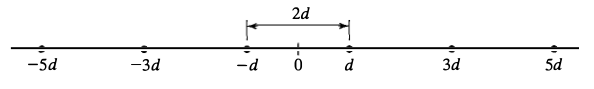
\includegraphics[width=5in]{../figures/fig8_41}
		\caption{The pulse levels are shown by dots on basis axis. Distance between any two pulses is $d$.}
		\label{fig:fig8_41}
	\end{figure}
	
	
	\begin{equation}\label{key}
	\begin{aligned}
	4d^2 
	&=\int_{-\infty}^\infty [ p(t)-(-p(t)) ]^2 dt\\
	&=\int_0^T (A-(-A) )^2 dt \\
	&=\int_0^T (2A )^2 dt \\
	&=4A^2 T
	\end{aligned}
	\end{equation}
	From here we get the value of $d$ and $d$ squared as follows
	
	\begin{equation}\label{eq:d2}
	d^2 = A^2 T
	\end{equation}
	Or
	\begin{equation}\label{eq:d}
	d=A\sqrt{T}
	\end{equation}
	Now we can write $\mathcal{E}_{avg}$ in Equation (\ref{eq:Eavg1}) in terms of $d$ as 
	
	\begin{equation}\label{eq:eavg}
	\mathcal{E}_{avg}=\frac{d^2 (M^2-1)}{3} \\
	\end{equation}
	Similarly, we can write $\mathcal{E}_{b}$ in Equation (\ref{eq:eb1}) terms of $d$ as 
	
	
	\begin{equation}\label{eq:eb}
	\mathcal{E}_{b}=\frac{d^2(M^2-1)}{3\log_2{M}}
	\end{equation}
	
	We can write $d^2$ in terms of $\mathcal{E}_{avg}$ and $\mathcal{E}_{b}$
	
	\begin{equation}\label{eq:dinEavg}
	d^2=\frac{3\mathcal{E}_{avg}}{(M^2-1)}
	\end{equation}
	
	
	\begin{equation}\label{eq:dinEb}
	d^2=\frac{3\mathcal{E}_{b}\log_2{M}}{(M^2-1)}
	\end{equation}
	
	
	\subsection{Probability of Error in PAM}
	
	The PAM modulated signal is received by the correlation detector
	
	The received signal is $r(t)$
	
	This is the sum of symbol waveform and the channel Additive White Gaussian Noise (AWGN)
	
	\begin{equation}\label{key}
	r(t)=s_m(t)+n(t)
	\end{equation}
	
	Or if the waveform is represented in the form of its basis function $\psi(t)$
	\begin{equation}\label{eq:rtbasis}
	r(t)=s_m \psi(t)+n(t)
	\end{equation}
	
	The AWGN noise is modeled by a Gaussian random variable.
	
	A Gaussian random variable is described completely by two parameters, its mean, $\mu$ and its variance $\sigma^2$
	
	\begin{equation}\label{eq:fnormal}
	f(x)=\frac{1}{\sqrt{2\pi \sigma_x^2}} e^{ -\frac{(x-\mu_x)^2}{2\sigma_x^2}}
	\end{equation}
	
	AWGN is the Gaussian R.V. with zero mean, $\mu_n=0$ and variance $\sigma_x^2=N_0/2$
	
	\begin{equation}\label{eq:fawgn}
	\begin{aligned}
	f(n)
	&=\frac{1}{\sqrt{2\pi N_0/2}} e^{-\frac{(n-0)^2}{2 (N_0/2)}}\\
	&=\frac{1}{\sqrt{\pi N_0}} e^{-\frac{n^2}{N_0}}
	\end{aligned}
	\end{equation}
	
	$N_0/2$ is the power spectral density of the noise measured in Watts/Hz
	
	The AWGN noise power is uniformally distributed our complete frequency band, hence it got the name white. White light contains all the wavelengths (frequencies) of light. 
	
	The signal power can be computed in three ways
	
	From its time description as
	
	\begin{equation}\label{key}
	\mathcal{P}_x = \lim_{T\rightarrow\infty}\frac{1}{T} \int_{-T/2}^{T/2} |x(t)|^2 dt
	\end{equation}
	
	From its frequency domain representation as 
	
	\begin{equation}\label{key}
	\mathcal{P}_x = \lim_{T\rightarrow\infty}\frac{1}{T} \int_{-\infty}^{\infty} |X(f)|^2 df
	\end{equation}
	where $X(f)$ is the Fourier transform of $x(t)$
	
	From its statistical properties as
	
	\begin{equation}\label{key}
	\mathcal{P}_x =  \mathbf{E}[X^2] = \int_{-\infty}^{\infty} x^2 f(x) dx
	\end{equation}
	where $x$ is the random variable and $f(x)$ is its probability density function.
	
	{\color{blue}
		\textbf{Homework:} Compute the signal power of the pulse train shown in Figure \ref{fig:fig227}, having peak amplitude $A$ and period $T$ from its time domain, frequency domain and probabilistic representations for following cases
		
		\begin{figure}
			\centering
			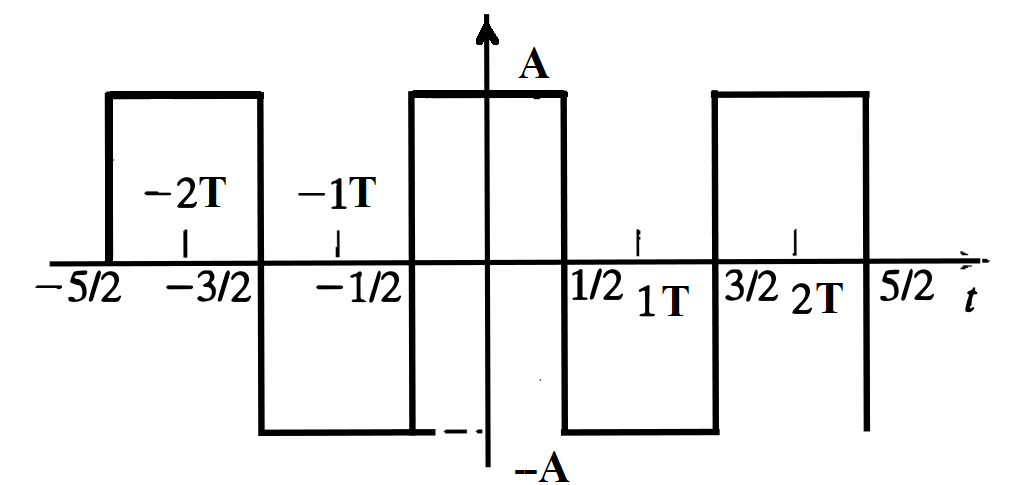
\includegraphics[width=2.7in]{../figures/fig2_27}
			\caption{Find pulse train power from its time, frequency and statistical properties}
			\label{fig:fig227}
		\end{figure}
		
		1) When the pulses amplitudes are $0$ and $A$
		
		2) When the pulses amplitude are $-A/2$ and $A/2$
	}
	
	Greater the noise power $N_0$, greater the spread of the noise values about zero.
	
	\subsubsection*{Why the Gaussian noise?}
	
	There are two reasons
	
	1) There is large portion of thermal noise in communication systems. Heated electronics components produce white noise, both at transmitter and receiver side. It is modelled as noise added by the channel. Thermal noise has Gaussian distribution.
	
	2) Due to central moment theorem, if multiple random processes add up, their cumulative probability density function is Gaussian distribution.
	
	The correlation type detector applies the following operations on received signal $r(t)$
	
	\begin{equation}\label{key}
	r(t)=s_m \psi(t)+n(t)
	\end{equation}
	This received signal is then multiplied with the basis function to get $x(t)$
	
	\begin{equation}\label{key}
	\begin{aligned}
	x(t)
	&=(s_m \psi(t)+n(t))\psi(t) \\
	&=s_m \psi^2(t)+n(t)\psi(t)
	\end{aligned}
	\end{equation}
	

	
	Next this signal is passed through an integrator to get $y(t)$
	
	\begin{equation}\label{key}
	\begin{aligned}
	y(t)
	&=\int_0^t x(t)dt \\
	&=\int_0^t (s_m \psi(t)+n(t))\psi(t)dt \\
	&=\int_0^t s_m \psi^2(t)dt + \int_0^t n(t)\psi(t) dt
	\end{aligned}
	\end{equation}
	
	Next the signal $y(t)$ is sampled at end of the symbol time, $T$
	
	\begin{equation}\label{eq:y}
	\begin{aligned}
	y=y(T)
	&=s_m \int_0^T \psi^2(t)dt + \int_0^T n(t)\psi(t) dt \\
	&=s_m+n
	\end{aligned}
	\end{equation}
	
		\begin{figure}
		\centering
		\includegraphics[width=\linewidth]{../figures/AWGNChannel}
		\caption{Cross correlator for M-PAM modulated signals.}
		\label{fig:fig820}
	\end{figure}

	where we used the face that energy of basis is one. $n$ is the correlation of n(t) along the basis function. It is a sample of the AWGN Gaussian random variable and has mean $\mu_n=0$ and $\sigma_n=N_0/2$ 
	
	
	\begin{equation}\label{key}
	n=\int_0^T n(t) \psi(t) dt
	\end{equation}
	
	Now $y$ is a new random variable. $s_m$ is a constant which is inner product of $s_m(t)$ with basis function $\psi(t)$.
	
	\begin{equation}\label{eq:muy}
	\begin{aligned}
	\mu_y
	&=\mathbf{E}[y] \\
	&=\mathbf{E}[s_m+n] \\
	&=\mathbf{E}[s_m]+\mathbf{E}[n] \\
	&=s_m+\mathbf{E}[n] \\
	&=s_m+\mu_n
	\end{aligned}
	\end{equation}
	
	where we use the fact that expected value of a constant value is that constant value.
	
	Since $\mu_n=0$
	
	\begin{equation}\label{key}
	\mu_y=s_m
	\end{equation}
	
	The variance of $y$ is
	\begin{equation}\label{eq:sigmay}
	\begin{aligned}
	\sigma^2_y
	&=\mathbf{E}[(y-\mu_y)^2] \\
	&=\mathbf{E}[(s_m+n-s_m)^2] \\
	&=\mathbf{E}[n^2] \\
	&=\mathbf{E}[n^2]-0 \\
	&=\mathbf{E}[n^2]-(\mathbf{E}[n])^2 \\
	&=\sigma_n^2 \\
	&=N_0/2
	\end{aligned}
	\end{equation}
	
	where we used the definition of variance as $Var(y)=\mathbf{E}[(y-\mu_y)^2] $.
	
	The sampled $y$ is a Gaussian random variable haveing mean $s_m$ and variance $\sigma_n^2=N_0/2$. The probability density function of $y$ is a bell curve centred at $s_m$.
	
	\begin{equation}\label{}
	\begin{aligned}
	f(y)
	&=\frac{1}{\sqrt{\pi N_0}} e^{-\frac{(y-s_m)^2}{N_0}}
	\end{aligned}
	\end{equation}
	
	The function of the detector is to map received $y$ to the symbol used at receiver $s_m$.
	
	Though $y$ has high probability to be near its mean value of $s_m$ but there is non zero probability that its value is far off from $s_m$.
	
	If the $y$ is within $d$ distance of the mean value, then it would be correctly detected as $s_m$. We calculated $d$ earlier in Equation (\ref{eq:d}.)
	
	If $y$ is below its mean value then receiver will make a mistake and consider it $s_{m-1}$. Also if $y$ is above its mean value more than $d$, then receiver will make a mistake and consider it $s_{m+1}$
	
	For the smallest pulse $s_1(t)$ the error is half of others. Error is only made when $y$ is greater than $s_1+d$. If $y$ is less than $s_1-d$ no mistake is made as every value below $s_1$ is correctly detected as $s_1$.
	
	Similiar is the case for the highest pulse as its error occurs only when $y$ is less than $s_m-d$ and no error is made if $y>(s_m+d)$
	
	Therefore the probability of error for the two pulses at extremes is half of the error for all other pulses
	
	The error is calculated by integrating the received random variable in the undesired region.
	
	The probability of error when $s_1$ is transmitted is given by
	
	\begin{equation}\label{eq:pe1}
	\begin{aligned}
	P_{e1}
	&=P(y>d)\\
	&= \int_d^\infty f(y)dy\\
	&= \int_d^\infty \frac{1}{\sqrt{\pi N_0}} e^{-\frac{(y-s_m)^2}{N_0}} dy\\
	\end{aligned}
	\end{equation}
	
	\begin{figure}
		\centering
		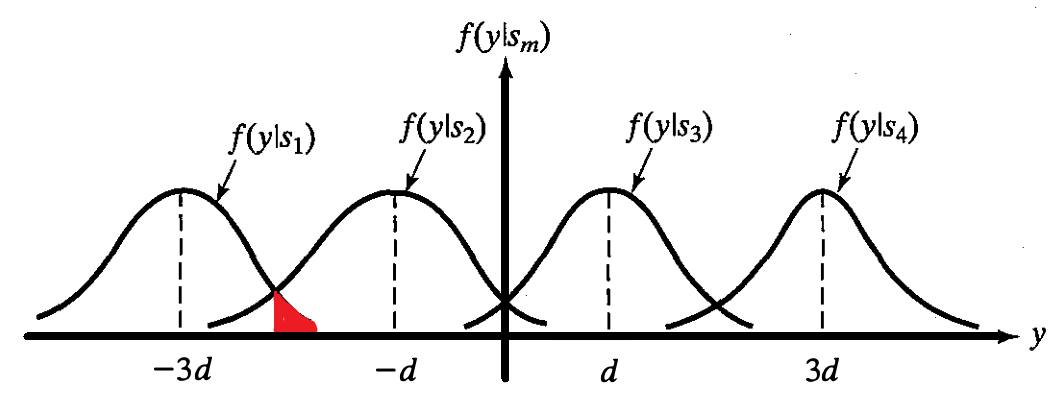
\includegraphics[width=\linewidth]{../figures/fig8_37}
		\caption{PDFs for M = 4 received PAM signals in additive white Gaussian noise. For signal $s_1$ detection error $P_{e1}$ is made in the red region.}
		\label{fig:fig837}
	\end{figure}
	
	
	So the error can be calculated by evaluating the integral in Equation (\ref{eq:pe1})). Unfortunately, however, does not have any closed form. We have only tables available for standard normal random variable  probability cumulative density functions (CDF). Som eof the popular CDF functions are given below.
	
	
	
	
	\[
	{\displaystyle \Phi (x)={\frac {1}{\sqrt {2\pi }}}\int _{-\infty }^{x}e^{-t^{2}/2}\,dt}
	\]
	
	
	\[
	{\displaystyle Q(x)={\frac{1}{\sqrt {2\pi }}}\int _{x}^{\infty}e^{-t^{2}/2}\,dt}
	\]
	
	
	\[
	{\displaystyle \operatorname {erf} (x)={\frac {2}{\sqrt {\pi }}}\int _{0}^{x}e^{-t^{2}}\,dt}
	\]
	
	\[
	{\displaystyle \operatorname {erfc} (x)={\frac {2}{\sqrt {\pi }}}\int _{x}^{\infty}e^{-t^{2}}\,dt}
	\]
	
	Communication systems books usually use the error-function and complementary-error-function tables. For statistics literature, the $\Phi(x)$ function is usually used. One other popluar choice is $Q(x)$ function which is also the one used by our text book. So we make error calculations using $Q$-function.
	
	The $Q(x)$ tables the probablity $P(X>x)$ of a zero mean $\mu_x=0$ and unit variance $\sigma_x^2=1$ Gaussian random variable to have value greater than $x$.
	
	\begin{equation}\label{key}
	\begin{aligned}
	Q(x)&=  P(X>x)\\
	&=\frac{1}{\sqrt{2\pi}} \int_x^\infty e^{-t^2/2} dt \\
	\end{aligned}
	\end{equation}
	
	With small change if variables we can also see the following definition of $Q(x)$
	
	\begin{equation}\label{key}
	\begin{aligned}
	Q(x) &= P(X<-x) \\
	&=\frac{1}{\sqrt{2\pi}} \int_{-\infty}^x e^{-t^2/2} dt \\
	\end{aligned}
	\end{equation}
	
	Few points to note for Q(x) are
	
	\begin{equation*}\label{key}
	\begin{aligned}
	Q(0)&=0.5\\
	Q(-x)&=1-Q(x)\\
	Q(\infty)&=0\\
	Q(-\infty)&=1
	\end{aligned}
	\end{equation*}
	
	If we have to evaluate $P(y>d)$ for a normal random variable with mean $\mu$ and variance $\sigma^2$
	
	
	
	%Now we go back to our Equation (\ref{eq:pe1}) and proceed
	%
	\begin{equation*}\label{}
	\begin{aligned}
	P(y>d)
	&= \int_d^\infty f(y)dy\\
	&= \int_d^\infty \frac{1}{\sqrt{2\pi \sigma^2}} e^{-(y-\mu)^2/ 2\sigma^2} dy\\
	\end{aligned}
	\end{equation*}
	
	Let us make variable changes in above equation
	
	\begin{equation}\label{eq:y2x}
	\begin{aligned}
	\frac{x^2}{2}&=\frac{(y-\mu)^2}{2\sigma^2}\\
	\implies x^2&=\frac{(y-\mu)^2}{\sigma^2} \\
	\implies x&=\frac{(y-\mu)}{\sigma} \\
	\end{aligned}
	\end{equation}
	
	Differentiating Equation (\ref{eq:y2x})
	
	\begin{equation}\label{key}
	\begin{aligned}
	dx &= \frac{1}{\sigma} dy \\
	\implies  dy &= \sigma dx
	\end{aligned}
	\end{equation}
	
	Also the limits will be changed
	
	\begin{equation}\label{key}
	\begin{aligned}
	y=d &\implies x=\frac{d-\mu}{\sigma}\\
	y=\infty &\implies x=\frac{\infty-\mu}{\sigma}=\infty\\
	\end{aligned}
	\end{equation}
	
	\begin{equation}\label{eq:y2Q}
	\begin{aligned}
	P(y>d)
	&= \int_d^\infty \frac{1}{\sqrt{2\pi \sigma^2}} e^{-(y-\mu)^2/ 2\sigma^2} dy\\
	&= \int_{\frac{d-\mu}{\sigma}}^\infty \frac{1}{\sqrt{2\pi \sigma^2}} e^{x^2/2} \sigma dx\\
	&= \int_{\frac{d-\mu}{\sigma}}^\infty \frac{1}{\sqrt{2\pi}} e^{x^2/2}dx\\
	&=Q(\frac{d-\mu}{\sigma})
	\end{aligned}
	\end{equation}
	
	Hence probability of error can be calculated for any Gaussian random variable using the $Q(x)$ function.
	
	Now we are able to complete Equation (\ref{eq:pe1}) to calculate $P(y>d)$. We have earlier calculated the mean value of y, $\mu_y$ in Equation (\ref{eq:muy}) and its variance $\sigma_y$  in Equation (\ref{eq:sigmay}). Substituting these values in Equation (\ref{eq:y2Q}) we calculate the error probability in terms of Q(x).
	
	\begin{equation}\label{eq:pe1b}
	\begin{aligned}
	P_{e1}
	&=P(y>d)\\
	&=Q(\frac{d-0}{\sqrt{N_0/2}}) \\
	&=Q(\sqrt{\frac{2d^2}{N_0}})
	\end{aligned}
	\end{equation}
%	
%	Now using the value of $d^2$ calculated in Equation (\ref{eq:d2}) in above equation we get
%	
%	\begin{equation}\label{eq:pe1c}
%	\begin{aligned}
%	P_{e1}
%	&=P(y>d)\\
%	&=Q\left(\frac{d-0}{\sqrt{N_0/2}}\right) \\
%	&=Q\left(\sqrt{\frac{2d^2}{N_0}}\right)
%	\end{aligned}
%	\end{equation}
%	
	$P_{e1}$ is the error in detection when $s_1(t)$ was transmitted. By symmetry, the probability of error when $s_M(t)$ is transmitted is also $P_{e1}$. For each of the other $(M-2)$ pulses, the probability of error is twice that, i.e. $2P_{e1}$. If each symbol is equiprobable, probability of occurance of one symbol is $1/M$. 
	\begin{equation}\label{key}
	P(s_1(t))=P(s_2(t))=\cdots=P(s_M(t))=1/M
	\end{equation}
	
	So the average probability of error per symbol is
	
	\begin{equation}\label{key}
	\begin{aligned}
	P_e 
	&= P(s_1) P_{e1}+P(s_2) (2P_{e1})+\cdots+P(s_{M-1}) (2P_{e1})+P(s_M) P_{e1} \\
	&= \frac{ P_{e1}+ 2P_{e1}+\cdots+ 2P_{e1}+ P_{e1})}{M} \\
	&=\frac{2(M-1)}{M}P_{e1}
	\end{aligned}
	\end{equation}
	
	Substituting the value of $P_{e1}$ from Equation (\ref{eq:pe1})
	
	\begin{equation}\label{key}
	\begin{aligned}
	P_e 
	&=\frac{2(M-1)}{M} Q\left(\sqrt{\frac{2d^2}{N_0}}\right)
	\end{aligned}
	\end{equation}
	
	Using Equation (\ref{eq:dinEavg}) we obtain error probability as 
	
	\begin{equation}\label{key}
	\begin{aligned}
	P_e 
	&=\frac{2(M-1)}{M} Q\left(\sqrt{\frac{6\mathcal{E}_{avg}}{N_0(M^2-1)}}\right)
	\end{aligned}
	\end{equation}
	
	The symbol error probability in terms of bit energy 
	$\mathcal{E}_{b}$ derived in Equation (\ref{eq:dinEb}) is
	
	\begin{equation}\label{key}
	\begin{aligned}
	P_e 
	&=\frac{2(M-1)}{M} Q\left(\sqrt{\frac{6\mathcal{E}_{b}\log_2 M}{N_0(M^2-1)}}\right)
	\end{aligned}
	\end{equation}
	
	\begin{figure}
		\centering
		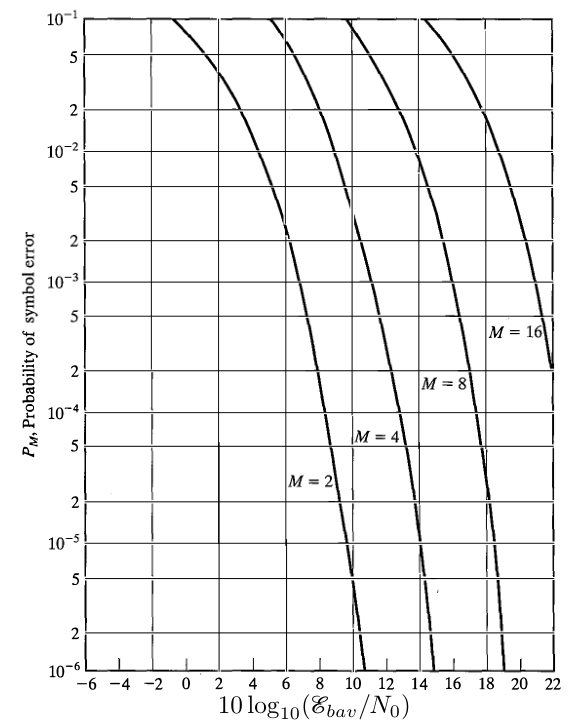
\includegraphics[width=.7\linewidth]{../figures/fig8_46}
		\caption{The probability of a symbol error as a function of $10\log_{10}(\mathcal{E}_{bav}/N_0)$ in dB for $M=2,4,8,16$.}
		\label{fig:fig846}
	\end{figure}
	
	\subsection{Homework and Reading}



	\begin{itemize}
		\item TEXT BOOK: FUNDAMENTALS OF COMMUNICATION SYSTEMS by John G. Proakis and 		Masoud Salehi, Second Edition
\item CHAPTER 8, DIGITAL MODULATION METHODS IN AN ADDITIVE WHITE GAUSSIAN NOISE CHANNEL
\item 8.4 M-ary Digital Modulation 
\item 8.4.1 The Optimum Receiver for M-qry Signals in AWGN
\item 8.4.2 A Union Bound on the Probability of Error
\item 8.5 M-ary Pulse Amplitude Modulation
\item 8.5.1 Carrier-Modulated PAM for Bandpass Channels (M-ary ASK)
\item 8.5.2 Demodulation and Detection of Amplitude-Modulated PAM Signals
\item 8.5.3 Probability of Error/or M-ary PAM
		\item End Problems: P8.13, P8.14,P8.19, P8.20, P8.22, P8.23
	\end{itemize}
\end{document}
